%%%%%%%%%%%%%%%%%%%%%%%%%%%%%%%%%%%%%%%%%%%%%%%%%%%%%%%%%%%%%%%%%%%%%%%%%%%%%%%
%% 3.- PROGRAMA UTA
%%%%%%%%%%%%%%%%%%%%%%%%%%%%%%%%%%%%%%%%%%%%%%%%%%%%%%%%%%%%%%%%%%%%%%%%%%%%%%%

\cleardoublepage
\chapter{Programa Unidad de Tratamiento de Aire}
\chaptermark{Programa Unidad de Tratamiento de Aire}

\label{chap:anexoProgramaUTA} % etiqueta para poder referenciar luego en el texto con ~\ref{sec:intro}
% \addcontentsline{toc}{chapter}{Introducción, Objetivos, Metodología y Planificación

\begin{figure}[H]
    \centering
    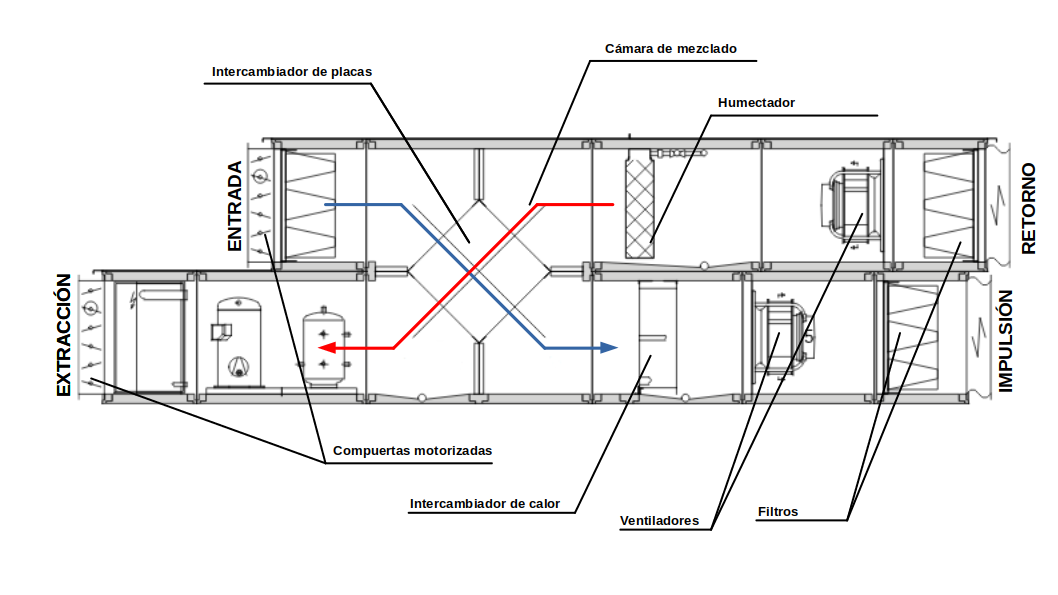
\includegraphics[width=\textwidth, keepaspectratio]{img/esquemaUTA}
    \caption{Plano de partes de una UTA}
    \label{figura:sasssssd}
\end{figure}

El programa para el control de la UTA se ha realizado el software ISaGRAF, que emplea los lenguajes de estándar IEC61131:                   

\begin{itemize}
    \item (\textbf{LD}) Escalera  
    \item (\textbf{FBD}) Diagrama a Bloques 
    \item (\textbf{SFC}) Tabla de Funciones Secuenciales 
    \item (\textbf{ST}) Texto Estructurado 
    \item (\textbf{IL}) Lista de Instrucciones 
    \item (\textbf{FC}) Diagrama de flujo 
  \end{itemize}

El programa se compone de una parte de configuración de entradas, salidas, parámetros, alarmas y warnings, y otra parte dedicada a la programación del funcionamiento de la UTA.

En este anexo se muestran las variables configuradas (\hyperref[tab:variablesUTA]{Tabla~\ref{tab:variablesUTA}}), y la lógica de funcionamiento programada.

\begin{center}
    \begin{longtable}{|p{2.2cm}|p{5.3cm}|p{7cm}|}
    
    
    \hline \cellcolor{lightgray}\centering\textbf{GRUPO} & \cellcolor{lightgray}\centering\textbf{VARIABLE} & \cellcolor{lightgray}\textbf{DESCRIPCIÓN} \\ \hline 
    \endfirsthead
    
    \multicolumn{3}{c}%
    {\footnotesize{\bfseries \tablename\ \thetable{} ...continuación de la página anterior.}} \\
    \hline \cellcolor{lightgray}\textbf{GRUPO} & \cellcolor{lightgray}\textbf{PARÁMETRO} & \cellcolor{lightgray}\textbf{DESCRIPCIÓN} \\ \hline 
    \endhead
    
    \hline  \multicolumn{3}{c}%
    {\footnotesize{\bfseries \tablename\ \thetable{} continua en la página siguiente...}} \\
    \endfoot
    
    \hline
    \caption{Variables configuración control} 
    \label{tab:variablesUTA}
    \endlastfoot
    
        \centering{Entradas} & \small\centering\textbf{Pb\_T\_IMP\_AIRE} & \small{Sonda de temperatura de impulsión de aire} \\ \cline{2-3}
        \centering{analógicas}& \small\centering\textbf{Pb\_T\_RET\_AIRE} & \small{Sonda de temperatura de retorno de aire} \\ \cline{2-3}
        & \small\centering\textbf{Pb\_T\_IMP\_AGUA} & \small{Sonda de temperatura de impulsión de agua} \\ \cline{2-3}
        & \small\centering\textbf{Pb\_T\_RET\_AGUA} & \small{Sonda de temperatura de retorno de agua} \\ \cline{2-3}
        & \small\centering\textbf{Pb\_T\_EXTRAC\_AIRE} & \small{Sonda de temperatura de extracción de aire} \\ \cline{2-3}
        & \small\centering\textbf{Pb\_T\_EXT\_AIRE} & \small{Sonda de temperatura de aire exterior} \\ \cline{2-3}
        & \small\centering\textbf{Pb\_H\_RET} & \small{Sensor de humedad de aire de retorno} \\ \cline{2-3}
        & \small\centering\textbf{Pb\_H\_EXT} & \small{Sensor de humedad de aire exterior} \\ \hline

        \centering{Entradas} & \small\centering\textbf{DI\_ONOFF} & \small{Interruptor de ON/OFF remoto} \\ \cline{2-3}
        \centering{digitales} & \small\centering\textbf{DI\_VENT\_IMP} & \small{Seguridad ventilador de impulsión} \\ \cline{2-3}
        & \small\centering\textbf{DI\_VENT\_RET} & \small{Seguridad ventilador de retorno} \\ \cline{2-3}
        & \small\centering\textbf{DI\_NIVEL\_HUM} & \small{Indicador nivel humectador lleno} \\ \hline

        \centering{Salidas} & \small\centering\textbf{RELE\_VALVE3V} & \small{Válvula de recirculación de agua desde central} \\ \cline{2-3}
        \centering{digitales} & \small\centering\textbf{RELE\_HUMECT} & \small{ON/OFF humectador} \\ \cline{2-3}
        & \small\centering\textbf{RELE\_ALARM} & \small{ON/OFF alarma} \\ \hline

        \centering{Salidas} & \small\centering\textbf{AO\_VENT\_IMP} & \small{Regulación velocidad ventilador impulsión} \\ \cline{2-3}
        \centering{analógicas} & \small\centering\textbf{AO\_VENT\_RET} & \small{Regulación velocidad ventilador retorno} \\ \hline

        \centering{Alarmas} & \small\centering\textbf{ALARM\_VENT\_IMPULSION} & \small{Alarma en ventilador de impulsión} \\ \cline{2-3}
        & \small\centering\textbf{ALARM\_VENT\_RETORNO} & \small{Alarma en ventilador de retorno} \\ \hline

        \centering{Warnings} & \footnotesize\centering\textbf{WARNING\_VENT\_IMPULSION} & \small{Aviso de fallo en ventilador de impulsión} \\ \cline{2-3}
        & \footnotesize\centering\textbf{WARNING\_VENT\_RETORNO} & \small{Aviso de fallo en ventilador de retorno} \\ \cline{2-3}
        & \footnotesize\centering\textbf{WARNING\_FILTRO\_ENTRADA} & \small{Aviso de filtro de entrada sucio} \\ \cline{2-3}
        & \footnotesize\centering\textbf{WARNING\_FILTRO\_IMPULSION} & \small{Aviso de filtro de impulsión sucio} \\ \cline{2-3}
        & \footnotesize\centering\textbf{WARNING\_FILTRO\_RETORNO} & \small{Aviso de filtro de retorno sucio} \\ \cline{2-3}
        & \small\centering\textbf{WARNING\_H\_FLUID\_TMP} & \small{Aviso de temperatura alta en fluido para alcanzar consigna} \\ \cline{2-3}
        & \small\centering\textbf{WARNING\_L\_FLUID\_TMP} & \small{Aviso de temperatura baja en fluido para alcanzar consigna} \\ \hline
    \end{longtable}
\end{center} 

\clearpage

\vspace*{\fill}

\begin{figure}[H]
    \centering
    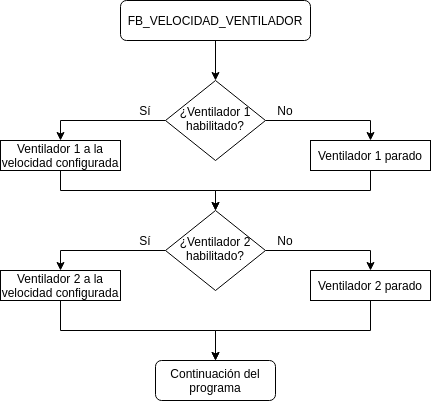
\includegraphics[width=0.8\textwidth, keepaspectratio]{img/0-fbVelocidadVentilador}
    \caption{Flujo de programa para gestión de ventiladores}
    \label{figura:gestionVentiladores}
\end{figure}

   \vspace*{\fill}

La \hyperref[figura:gestionVentiladores]{Figura~\ref{figura:gestionVentiladores}~anterior} muestra el flujo de programa para la función encargada de analizar si los ventiladores están habilitados y sin fallos, para enviarles la velocidad deseada. Esta función será llamada desde el módulo encargado de decidir qué velocidad es la deseada en los ventiladores (\hyperref[figura:gestionVelocidadVentiladores]{Figura~\ref{figura:gestionVelocidadVentiladores}}): la velocidad puede ser baja, media, alta o el resultado del control automático de la \hyperref[figura:gestionAutomatica]{Figura~\ref{figura:gestionAutomatica}}. 

Por último, el humectador se controla según la lógica de la \hyperref[figura:gestionHumectador]{Figura~\ref{figura:gestionHumectador}}.

\clearpage 

   \vspace*{\fill}

\begin{figure}[H]
    \centering
    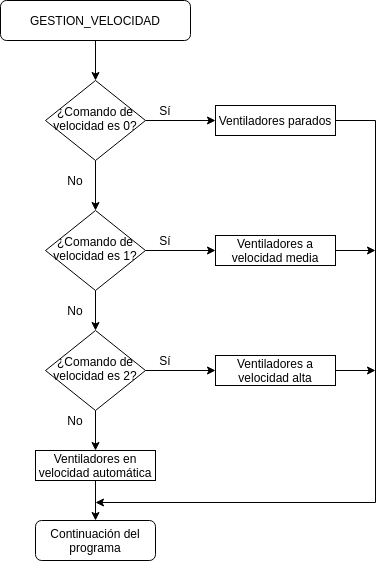
\includegraphics[width=0.7\textwidth, keepaspectratio]{img/1-gestionVelocidad}
    \caption{Flujo de programa de gestión de la velocidad}
    \label{figura:gestionVelocidadVentiladores}
\end{figure}

   \vspace*{\fill}

\clearpage  

   \vspace*{\fill}

\begin{figure}[H]
    \centering
    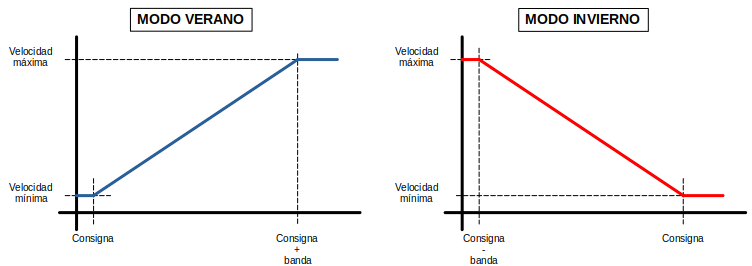
\includegraphics[width=\textwidth, keepaspectratio]{img/2-gestionAutomatica}
    \caption{Curvas de control automático de la velocidad en ventiladores, en función de la temperatura}
    \label{figura:gestionAutomatica}
\end{figure}
  
   \vspace*{\fill}

\begin{figure}[H]
    \centering
    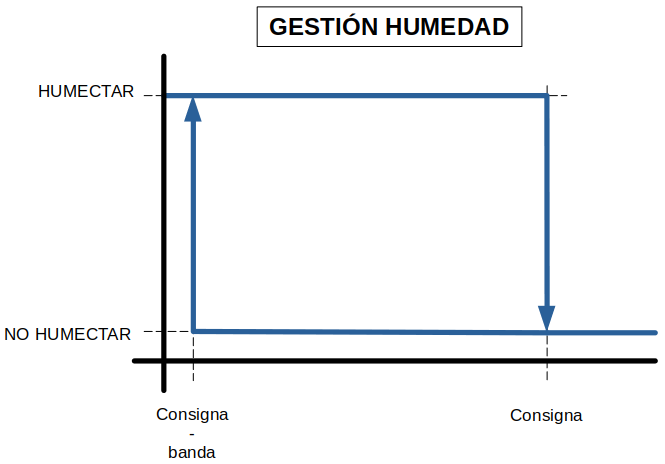
\includegraphics[width=0.5\textwidth, keepaspectratio]{img/3-gestionHumedad}
    \caption{Curva de control del humectador}
    \label{figura:gestionHumectador}
\end{figure}

   \vspace*{\fill}


